\documentclass{../src/bcthesispart}
\title{Lateral Inhibition Strategies}
\author{Bas Cornelissen}
\begin{document}

%——————————————————————————————————————————————————————————
\appendixtitle{Lateral Inhibition Strategies}{Lateral Inhibition Strategies}{li-strategies}{%
	%
	% Abstract
	% ————————
	In chapter \ref{ch:naming-games} we explored five different lateral inhibition strategies, and concluded that they always converge to an effective, shared language.
	Do these conclusions indeed generalize to the rest of the 6-dimensional, strategy space?
	The convergence proof suggests so, but does not apply to the naming games directly. 
	In this appendix part of the parameter space is therefore explored systematically.
	The results indicate that effective languages eventually emerge for all strategies, although the dynamics before convergence can vary substantially.
}
%——————————————————————————————————————————————————————————


\noindent
Recall that the space of lateral inhibition strategies is defined by five nonnegative parameters
\begin{equation}
	\delta_{\text{inc}}, \quad
	\delta_{\text{inh}}, \quad
	\delta_{\text{dec}}, \quad
	s_{\text{init}}, \quad 
	s_{\text{max}}.	
\end{equation}
I have not been able to find a systematic analysis of the parameter space.
\textcite{Wellens2012} does compare several strategies and suggest that the the value of the parameters determines the strategy. 
For example concluding that “a higher value [of $\delta_{\text{inh}}$] improves alignment”.
I belief this is slightly inaccurate, since the strategies are invariant under scaling.
In other words, it is the \emph{relative} value of the parameters that matters.
There are many more such equivalences.
%Translating $\delta_{\text{init}}, s_{\text{min}}$ and $s_{\text{max}}$ for example does not alter a strategy.
One could for example use any other
$\delta_{\text{inh}} \ge s_{\text{init}}$ without altering the minimal strategy; or fix $s_{\text{max}} := s_{\text{init}}$ and use any $\delta_{\text{inc}}>0$.
Similarly, a different $\delta_{\text{inc}} > 0$ leaves the frequency strategy unchanged, since scores greater than $s_{\text{init}}$ are of the form $s_\text{init} + k\cdot \delta_{\text{inc}}$ and essentially track the frequency $k$ anyway.




%- - - - - - - -
\begin{SCfigure}
	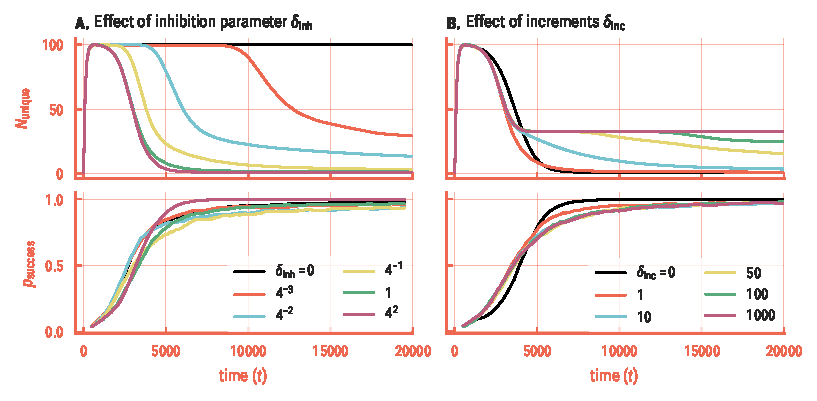
\includegraphics[trim=1.26cm 0 0 \figtopmargin]{LING03-02-combined-results}
	\caption{\subfig{A} The effect of $\delta_{\text{inh}}$ keeping $\delta_{\text{inc}} = 1$ fixed. It interpolates between the minimal strategy and frequency strategy. \subfig{B} the effect of $\delta_{\text{inc}}$ for $\delta_{\text{inh}} = 1$ fixed. For large $\delta_{\text{inc}}$, the inhibition is rendered ineffective.
		\figdetails{\figid{LING03}
		Results shown for $N=200$, $\delta_{\text{dec}} = 0$, $s_{\text{init}} = 1$, $s_{\text{max}} = \infty$; avg.\ of 300 runs. $p_{\text{success}}$ is moreover a rolling average over a centered window of 1000 iterations.
		}
		\label{fig:delta-inh-vs-delta-inc}}
\end{SCfigure}
%- - - - - - -




We map two slices of the strategy space by fixing either the increments or inhibition parameter and varying the other \parencite[following][]{Wellens2012}.
Figure \ref{fig:delta-inh-vs-delta-inc} reports the results.
Fixing $\delta_{\text{inc}} = 1$ while varying $\delta_{\text{inh}}$ (figure \ref{fig:delta-inh-vs-delta-inc}\textsc{a}) reveals that the inhibition parameter $\delta_{\text{inh}}$ interpolates between the minimal strategy ($\delta_{\text{inh}} = 4^2$ or larger; purple) and and the frequency strategy ($\delta_{\text{inh}} = 0$; black).
Both reach eventually reach perfect communicative success, but the stronger the lateral inhibition, the faster so.
The number of unique words $N_{\text{unique}}$ initially grows identically for all $\delta_{\text{inh}}$ as inhibition plays hardly any role at the start of the game.
In the frequency strategy, no words are ever removed and the resulting vocabulary is therefore not \emph{efficient}.
It is hard to tell if the amount of lateral inhibition matters in the long-term. The plot seems to suggest that this is not the case, and even the slightest lateral inhibition will (after a significantly longer time) result in a one-word language.




The effect of the increment $\delta_{\text{inc}}$ is shown in figure \ref{fig:delta-inh-vs-delta-inc}\textsc{b}.
One can see that the minimal strategy corresponds to $\delta_{\text{inc}} = 0$, but larger increments yield different dynamics.
After the peak of $N_{\text{unique}}$, words with score $\delta_{\text{init}} = 1$ are quickly removed, as it takes a single inhibition.
But words that have been heard multiple times have scores of at least $\delta_{\text{init}} + \delta_{\text{inc}}$ and need many more inhibitions to be removed.
There appear to be around $\nicefrac{N}{6}$ such words.
The result is a temporary stabilisation of $N_{\text{unique}}$.
Eventually inhibition takes over and competing words start disappearing. 
The (very) long-term behaviour thus appears to be the same as before: convergence to a single-word language.

%
%The take home message seems to be this: all strategies we have discussed give rise to a shared convention that allows the population to name the object.
%If there is any form of lateral inhibition, the stable language will have only a single word as all competing words will have been removed.
%Indeed, a shared single word language is a stable state: no words need to be invented and there are no words to inhibit.
%The only strategy with different stable states is the frequency strategy.
%There \emph{all} invented words spread the population, but since agents use the most frequent word, they can still communicate effectively.
%The precise dynamics leading to the stable stable state depends on the parameter settings.
%Communicative success can increase faster, slower or even stabilise temporarily, but will eventually be reached nonetheless.


%——————————————————————————————————————————————————————————
\showbibliography


\end{document}